\documentclass[tikz]{standalone}

\usetikzlibrary{decorations.pathmorphing}

\begin{document}
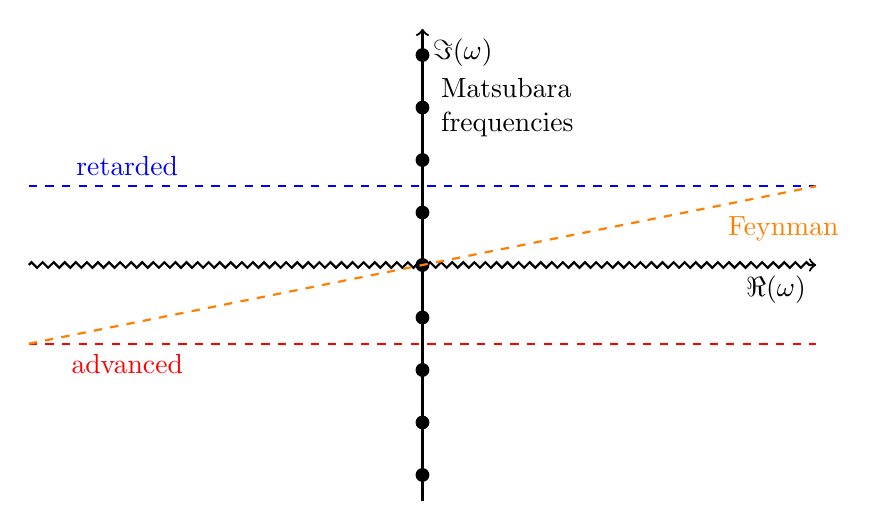
\begin{tikzpicture}[thick]

  % Axes
  \def\rerange{5}\def\imrange{4}
  \draw[->] [decorate,decoration={zigzag,segment length=4,amplitude=1,post=lineto,post length=2}] (-\rerange,0) -- (\rerange,0) node[below left] {$\Re(\omega)$};
  \draw[->] (0,-\imrange+1) -- (0,\imrange-1) node[below right] {$\Im(\omega)$};

  \foreach \n in {-\imrange,...,\imrange}{%
      \node[circle,fill,inner sep=0,minimum size=5] (omega\n) at (0,2/3*\n) {};}
  \node[right=3,align=left] (mf) at (omega3) {Matsubara\\frequencies};

  % Propagators
  \draw[red,dashed] (-\rerange,-1) -- (\rerange,-1) node[below,very near start] {advanced};
  \draw[blue,dashed] (-\rerange,1) -- (\rerange,1) node[above,very near start] {retarded};
  \draw[orange,dashed] (-\rerange,-1) -- (\rerange,1) node[below right,very near end] {Feynman};

\end{tikzpicture}
\end{document}